\documentclass{beamer}

\usetheme{Boadilla}

\newcommand{\bi}{\begin{itemize}}
\newcommand{\ei}{\end{itemize}}
\newcommand{\be}{\begin{enumerate}}
\newcommand{\ee}{\end{enumerate}}
\newcommand{\bc}{\begin{center}}
\newcommand{\ec}{\end{center}}
\newcommand{\bd}{\begin{description}}
\newcommand{\ed}{\end{description}}
\newcommand{\I}{\item}
\newcommand{\f}{\frame}
\newcommand{\ft}{\frametitle}

\title{Offline Software Status}
\subtitle{GlueX Collaboration Meeting}
\author[Mark Ito]{Mark M.\ Ito}
\date{October 3, 2019}
\institute[JLab]{Jefferson Lab}

\begin{document}

\f{\titlepage}

\f{\ft{Outline}
  \bi
  \I HDGeant4 Meetings
  \I halld\_recon version control and launches
  \I XROOTD server
  \I Crash fixes
  \I Event Generator Realism (EvtGen)
  \I Time-History Plots
  \I Upgraded Time-of-Flight software
  \I New database servers for use on the farm
  \I Summary/Conclusions
  \ei
}

\f{\ft{HDGeant4 Meetings}
  \bi
  \I Meetings continue
  \I Summer slowdown in activity
  \I Issues still being raised and studied
  \I Biggest differences seen in response of calorimeters to charged tracks,
  especially in timing.
  \I Compare HDG3 vs.\ HDG4 vs.\ real data
  \ei
}

\f{\ft{{\tt halld\_recon} Version Control and Launches}
  \bi
  \I Reconstruction launch creates REST data with one version of halld\_recon.
  \I Analysis launch uses REST data as input, creates ROOT trees, uses newer
  version of halld\_recon.
  \I Monte Carlo needs {\bf both} versions of halld\_recon. One to produce REST
  files, the other to produce trees.
    \bi
    \I Justin succinctly summarized the problem.
    \ei
  \I Implemented solution: new table to keep track of history of these pairs.
    \bi
    \I MCwrapper can read table, only allow valid pairs.
    \ei
  \ei
}

\f{\ft{XROOTD Server}
  \bi
  \I XROOTD server up and running on scosg16.jlab.org (the submit host)
  \I Allows streaming of files (no need to copy to remote disk)
  \I MCwrapper uses XROOTD to stream random triggers from JLab
  \I Next step: stream input data for reconstruction/analysis jobs
  \ei
}

\f{\ft{Crash Fixes}
  \bi
  \I Started as the ``crash in ST matching''
  \I Alex A. reported the problem. Sean, Beni, Simon, Justin, and David studied it. David diagnosed it.
    \bi
    \I Create an object from the heap in brun
    \I Use it in evnt
    \I Launch multiple event threads all with same pointer
    \I When thread ends, object gets deleted
    \I An early exiting thread leaves with the punch bowl
    \I Party ends abruptly (segfault)
    \I Blame assigned to the innocent
    \ei
  \I Bug pattern found in many plugins. Appears to have propagated via
  copy-and-paste. Sean scanned through plugins and fixed them.
  \I Crashes from multi-run analysis jobs similar: objects created at
  beginning of each run not propagated correctly. --Sean
  \ei
}

\f{\ft{Event Generator Realism (EvtGen)}
  \bi
  \I Sean brings in the EvtGen package ``industry standard''
  \I Better models for particle decays
  \I Uses text configuration files
  \I Implemented as post-processor for HDDM-formatted event files
  \ei
}

\f{\ft{Time-History Plots}
  \bi
  \I New package to keep track of time dependent quantities
  \I CSV files for data (this is on you)
  \I Text configuration files for plotting
  \ei
}

\f{\ft{Number of MySQL Server Connections}
$$
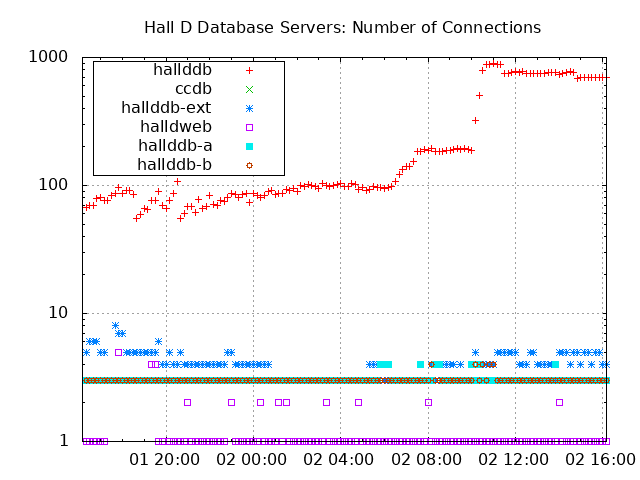
\includegraphics[width=3.5in]{mysql_servers_1.png}
$$
}

\f{\ft{Job Count, Currently Active Users}
$$
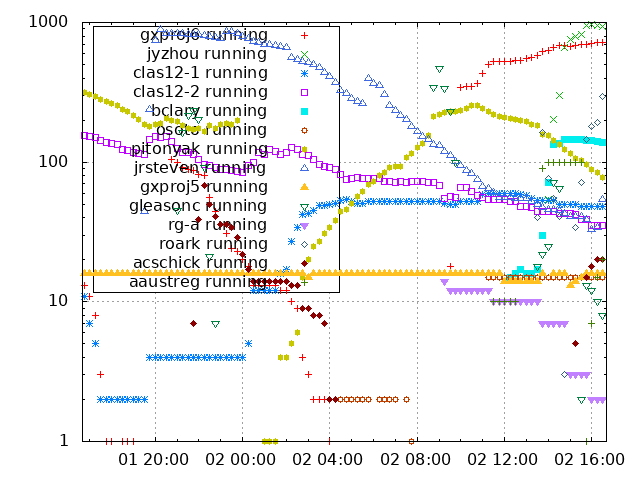
\includegraphics[width=3.5in]{user_jobs_1.png}
$$
}

\f{\ft{New Database Servers for Use on the Farm}
\bi
\I hallddb-farm.jlab.org
\I DNS alias for pair of new servers
\I Went into production this week
\ei
}

\f{\ft{Summary and Conclusions}
\bi
\I HDGeant4 in widespread use by the Collaboration
\I Need to get XROOTD streaming going
\I Documentation...
\ei
}

\end{document}
